\documentclass[conference]{IEEEtran}

% -------------------------------------------------------
% Packages
% -------------------------------------------------------
\usepackage{amsmath,amssymb}
\usepackage{graphicx}
\usepackage{booktabs}
\usepackage{multirow}
\usepackage{array}
\usepackage{tabularx}
\usepackage{rotating}
\usepackage{url}
\usepackage{tikz}
\usepackage{hyperref}
\usepackage{cite}
\usepackage{balance}
\usepackage{microtype}
\usepackage{times}
\usepackage[T1]{fontenc}
\usepackage{inputenc}
\usetikzlibrary{shapes.geometric, arrows, positioning, fit, calc}

\tikzstyle{block} = [rectangle, draw, fill=blue!10, text width=2.2cm, text centered, align=center, rounded corners, minimum height=1cm]
\tikzstyle{arrow} = [thick,->,>=stealth]
\tikzstyle{line} = [thick,-]
\hypersetup{
  colorlinks=true,
  linkcolor=blue,
  citecolor=blue,
  urlcolor=blue
}

% -------------------------------------------------------
% Helpers
% -------------------------------------------------------
\newcolumntype{C}[1]{>{\centering\arraybackslash}p{#1}}
\newcolumntype{L}[1]{>{\raggedright\arraybackslash}p{#1}}

% -------------------------------------------------------
% Title / Author
% -------------------------------------------------------
\title{Guardian 360: AI-Based Elderly Safety and Fall Risk Prediction
Wearable System Using CNN-GRU Architecture}

\author{
\IEEEauthorblockN{Dr.Anil B C}
\IEEEauthorblockA{
\textit{Professor and Head Department of CSE(AI \& ML)} \\
\textit{JSS Academy of Technical Education} \\
Bengaluru, India \\
hodaiml@jssateb.ac.in
}
\and
\IEEEauthorblockN{Abhinav Chandra. HS}
\IEEEauthorblockA{
\textit{Department of CSE(AI \& ML)} \\
\textit{JSS Academy of Technical Education} \\
Bengaluru, India \\
abhinavchandra@jssate.edu.in
}
\and
\IEEEauthorblockN{Dikshitha N}
\IEEEauthorblockA{
\textit{Department of CSE(AI \& ML)} \\
\textit{JSS Academy of Technical Education} \\
Bengaluru, India \\
dikshithan@gmail.com
}
\and
\IEEEauthorblockN{S V Preethi}
\IEEEauthorblockA{
\textit{Department of CSE(AI \& ML)} \\
\textit{JSS Academy of Technical Education} \\
Bengaluru, India \\
preethisv24@gmail.com
}
\and
\IEEEauthorblockN{Sahana H M}
\IEEEauthorblockA{
\textit{Department of CSE(AI \& ML)} \\
\textit{JSS Academy of Technical Education} \\
Bengaluru, India \\
sahanaa1215@gmail.com
}
}

% -------------------------------------------------------
\begin{document}
% -------------------------------------------------------

\maketitle

% -------------------------------------------------------
\begin{abstract}
Falls represent one of the most prevalent causes of injury and mortality
among elderly individuals worldwide, yet traditional monitoring systems
remain fundamentally reactive, detecting incidents only after they occur.
This paper presents \textbf{Guardian 360}, a novel AI-powered wrist-worn
embedded healthcare system that addresses the dual challenges of real-time
fall detection and proactive fall risk prediction for elderly individuals.
The system integrates a lightweight Convolutional Neural
Network--Gated Recurrent Unit (CNN-GRU) hybrid deep learning architecture
deployed directly on an ESP32 microcontroller, enabling on-device inference
from an MPU6050 Inertial Measurement Unit (IMU). The CNN stage extracts
discriminative local motion features from windowed accelerometer and
gyroscope data, while the GRU layer captures temporal gait dynamics and
progressive motion instabilities indicative of imminent fall risk.
Guardian~360 classifies continuous motion sequences into four categories:
\textit{Normal Gait}, \textit{Abnormal Gait}, \textit{Fall Risk}, and
\textit{Fall Event}, enabling caregivers to intervene before an injury
occurs. The wrist-worn device additionally monitors heart rate, blood
oxygen saturation (SpO$_2$), and body temperature via integrated sensors,
and incorporates GPS tracking, an SOS pushbutton, a piezoelectric buzzer,
and an OLED display. Emergency notifications are delivered to caregivers
through a Firebase IoT cloud pipeline. The proposed CNN-GRU model is
evaluated on the SisFall, MobiAct, and UP-Fall Detection benchmark datasets,
supplemented with collected gait sequences. Guardian~360 advances the state
of the art toward proactive, personalized, and embedded elderly healthcare.
\end{abstract}

\begin{IEEEkeywords}
Fall detection, fall risk prediction, gait analysis, CNN-GRU, wearable
sensor, elderly care, IoT, edge AI, TinyML, MPU6050, ESP32, predictive
healthcare, IMU, real-time monitoring
\end{IEEEkeywords}

% -------------------------------------------------------
\section{Introduction}
% -------------------------------------------------------

The global population of individuals aged 65 and above is projected to
reach 1.6 billion by 2050, placing an unprecedented burden on healthcare
systems worldwide~\cite{who2021falls}. Falls constitute the second leading
cause of accidental injury-related death globally, with approximately
684{,}000 fatal incidents occurring annually~\cite{ishaq2026}. Among
community-dwelling elderly individuals, one in three experiences at least
one fall per year, often resulting in fractures, prolonged hospitalization,
loss of independence, and a psychological fear of falling that further
accelerates physical decline~\cite{attal2015}.

Traditional elderly safety systems rely on manual clinical assessments,
fixed-threshold wearable alarms, and vision-based surveillance---all of
which are \textit{reactive}: they detect a fall only after it has occurred.
Recent advances in deep learning, edge AI, and miniaturized IoT sensors
have opened the possibility of \textit{predictive} monitoring systems
capable of identifying deteriorating gait patterns before an incident occurs.

Conventional wearable fall-detection systems predominantly employ Support
Vector Machines (SVM), Random Forest classifiers, or simple threshold
rules~\cite{kumar2024,zhang2025}. While effective for binary fall/no-fall
classification, these models cannot learn the temporal dependencies
inherent in gait-degradation sequences. Recurrent architectures such as
Long Short-Term Memory (LSTM) networks demonstrate improved sequential
modeling~\cite{gaud2025}, but their high memory footprint makes direct
deployment on resource-constrained microcontrollers impractical.

This paper proposes \textbf{Guardian~360}, integrating a CNN-GRU hybrid
architecture that balances predictive accuracy with computational
efficiency for edge deployment. The Gated Recurrent Unit
(GRU)~\cite{cho2014} achieves comparable temporal modeling to LSTM with
fewer parameters and lower memory requirements, making it the preferred
choice for TinyML deployment on the ESP32 microcontroller.

\subsection*{Primary Contributions}
\begin{itemize}
  \item A lightweight CNN-GRU model for four-class real-time gait and fall
        classification optimized for embedded microcontrollers.
  \item A comprehensive wearable IoT platform integrating IMU,
        photoplethysmography (PPG), GPS, and emergency-alerting subsystems.
  \item A proactive fall-risk prediction pipeline identifying unstable gait
        sequences \emph{before} a fall event occurs.
  \item Experimental validation on three public benchmark datasets.
  \item Full TensorFlow Lite deployment targeting sub-15\,ms inference on a
        240\,MHz dual-core microcontroller.
\end{itemize}

The remainder of this paper is organized as follows. Section~\ref{sec:lit}
reviews related literature. Section~\ref{sec:gap} identifies research gaps.
Section~\ref{sec:prob} states the problem. Section~\ref{sec:proposed}
describes the proposed system. Sections~\ref{sec:arch}--\ref{sec:dataset}
cover system architecture, methodology, the CNN-GRU model, and dataset
details. Sections~\ref{sec:hw}--\ref{sec:exp} describe hardware and
experimental setup. Section~\ref{sec:conclusion} concludes.

% -------------------------------------------------------
\section{Literature Survey}
\label{sec:lit}
% -------------------------------------------------------

\subsection{IoT-Based Remote Elderly Monitoring}

Bandara et al.~\cite{bandara2020} developed a comprehensive sensor platform
that integrated both wearable body-worn sensors and environmental IoT
devices deployed around the home, using the MQTT lightweight messaging
protocol for reliable real-time data transmission and cloud-based
visualization. The platform demonstrated consistent data acquisition across
multiple sensor modalities and showed promise for unobtrusive remote
monitoring; however, the system functioned purely as a data pipeline without
any layer of machine learning or predictive intelligence, meaning
caregivers could only react to raw readings rather than receive early
warnings of deteriorating health states.

Salma et al.~\cite{salma2025} conducted a rigorous PRISMA-guided scoping
review of Remote Monitoring Systems (RMS) designed for high-risk elderly
patients across multiple chronic conditions. Analysing dozens of peer-reviewed
studies, the authors found consistent evidence that continuous IoT-based
monitoring contributed to reduced rates of unplanned hospitalization and
improved adherence to care plans. Nonetheless, they cautioned that
significant heterogeneity in study design, sensor modalities, and outcome
measures made cross-study comparison difficult, and that no long-term
large-scale clinical validation of such systems existed at the time of
review.

Pasrija et al.~\cite{pasrija2025} presented a broad empirical argument for
the adoption of IoT-based continuous monitoring to support elderly
independence and improve emergency response times. Their work demonstrated
that remote connectivity between sensor nodes and caregiving staff could
substantially reduce the interval between an adverse event and a clinical
response; however, the authors themselves identified persistent and critical
gaps in AI-based predictive analytics, noting that existing deployments
were almost uniformly reactive rather than anticipatory in nature.

Mohammed and Hasan~\cite{mohammed2022} implemented a Raspberry Pi-based
smart healthcare monitoring system capable of reading and transmitting
physiological signals in near real-time, achieving approximately 97\%
heart-rate measurement accuracy under controlled conditions. The system
demonstrated that low-cost single-board computers could serve as
effective gateways for health data aggregation and cloud communication.
However, the platform was limited to physiological sensing and did not
incorporate any mechanism for fall detection, fall prediction, or movement
anomaly forecasting, making it unsuitable for safety-critical applications
where mobility and balance are the primary concern.

Augastiny et al.~\cite{augastiny2023} proposed a NodeMCU-based IoT health
monitoring system specifically designed for aged individuals, enabling
real-time tracking of temperature, pulse rate, and other physiological
parameters with automated alerts delivered via cloud platforms and mobile
applications. While the system offered convenient remote accessibility and
timely threshold-based notifications, it relied entirely on hard-coded
numerical thresholds for alert generation and incorporated no machine
learning models. As a result, it was inherently unable to detect nuanced
patterns indicative of progressive health deterioration or impending falls.

Ravikumar et al.~\cite{ravikumar2023} conducted a structured survey of
IoT-enabled Remote Patient Monitoring (RPM) systems, documenting their
positive impact on patient outcomes, reduction of unnecessary in-person
clinic visits, and overall healthcare cost reduction for chronic disease
management. The authors highlighted how real-time connectivity had begun
transforming post-acute care and home-based rehabilitation. Despite these
benefits, the survey noted the persistent absence of a unified, intelligent,
and deployment-ready solution that could seamlessly combine physiological
monitoring with AI-driven motion and gait analysis.

\subsection{Wearable Sensors and Activity Recognition}

Attal et al.~\cite{attal2015} conducted one of the most comprehensive
early comparative studies of supervised and unsupervised machine learning
techniques applied to human activity recognition using inertial measurement
unit data. The study evaluated k-Nearest Neighbour (k-NN), Support Vector
Machine (SVM), Random Forest, Gaussian Mixture Model (GMM), K-means
clustering, and Hidden Markov Model (HMM) classifiers on data collected
from six subjects performing twelve distinct activities of daily living
using three IMU sensors placed at the waist and wrists. The k-NN classifier
achieved the highest classification accuracy of approximately 99\% for
coarse activity classes; however, the work used entirely offline data,
lacked any real-time embedded deployment, and made no attempt to distinguish
deteriorating gait patterns or predict fall risk from the activity sequences.

Al-khafajiy et al.~\cite{alkhafajiy2019} proposed the Smart Wearable
Secure Health Monitoring System (SW-SHMS), a wearable IoT platform designed
for continuous remote monitoring of elderly patients. The system achieved
data transmission latency of less than 1\,ms under typical network
conditions, demonstrating the viability of low-latency wearable-to-cloud
pipelines for healthcare applications. The architecture used dedicated
hardware encryption for data security and a structured cloud storage
backend for caregiver access. Despite these engineering achievements, the
system focused exclusively on physiological parameters such as heart rate
and blood pressure, with no consideration of gait dynamics, movement
classification, or fall-related analysis.

Rahmani et al.~\cite{rahmani2024} introduced the EmoWear dataset, a
multimodal physiological and motion dataset collected from 49 participants
using a single wrist-worn device that simultaneously captured IMU
(accelerometer and gyroscope), electrocardiogram (ECG), blood volume pulse
(BVP), electrodermal activity (EDA), and respiration signals. The study
demonstrated that a single wrist-worn sensor unit could provide sufficient
signal diversity for simultaneous gait analysis, physical activity
recognition, and emotion state estimation, making a strong case for
multimodal wearables in holistic health monitoring. However, data collection
was performed in controlled laboratory settings, and no real-time inference
pipeline was developed or evaluated.

Saraubon et al.~\cite{saraubon2018} implemented a smart elderly-care system
using a combination of Raspberry Pi single-board computers, wrist-worn
accelerometers, and a convolutional neural network applied to acoustic
signals for fall detection. The system was one of the earlier examples of
deploying deep learning at the edge for elderly safety and achieved
approximately 93\% fall-detection accuracy on their experimental dataset,
demonstrating that accelerometer-based features consistently outperformed
acoustic features in detection reliability. Despite this contribution, the
system was designed exclusively to detect falls post-occurrence, offered
no predictive capability for identifying gait instability before a fall, and
did not incorporate any form of personalized monitoring or adaptation to
individual gait patterns.

\subsection{Fall Detection and Prediction Systems}

Gaud et al.~\cite{gaud2025} proposed FIBiLS, a deep learning pipeline
combining 1D Convolutional Neural Network and Bidirectional Long Short-Term
Memory (BiLSTM) layers for fall detection from dual IMU sensors, evaluated
on the SisFall benchmark dataset. The model processed both anterior and
posterior IMU channels simultaneously, exploiting bidirectional temporal
context to achieve 99.68\% detection accuracy with fast inference on a
standard computing platform. While FIBiLS represents one of the highest
reported detection accuracies in the fall-detection literature, the system
performs binary fall/no-fall classification only, with no mechanism to
recognize the progressive gait instability that precedes a fall. Furthermore,
the BiLSTM's parameter count and memory requirements rendered it unsuitable
for direct deployment on resource-constrained embedded devices such as the
ESP32 microcontroller.

Mekruksavanich et al.~\cite{mekruksavanich2022} applied aggregated residual
transformation networks---a multi-path convolutional architecture inspired
by ResNeXt---for automatic fall classification from wrist-worn IMU data. The
deep residual design allowed the network to learn complementary motion
features at multiple temporal scales, yielding improved classification
accuracy over conventional shallow convolutional baselines on simulated fall
data. The authors demonstrated that automatically learned deep representations
consistently outperformed hand-crafted statistical features; however, the
study was conducted entirely offline without any embedded deployment, and
the system classified only fall versus non-fall categories without addressing
the intermediate fall-risk state.

Zhang et al.~\cite{zhang2025} combined CNN and LSTM layers in a hybrid
architecture for temporal fall-pattern recognition from both wearable IMU
data and supplementary vision-based inputs, achieving high accuracy in
controlled indoor environments. The CNN extracted spatial motion features
from windowed sensor segments, while the LSTM captured the sequential
evolution of those features over time, enabling discrimination of complex
fall trajectories from ADL. The authors acknowledged, however, that the
absence of diverse real-world fall data severely limits generalizability,
and that the CNN-LSTM model's resource requirements precluded embedded edge
deployment, requiring cloud offloading for inference.

Ishaq et al.~\cite{ishaq2026} conducted a comprehensive PRISMA-based
systematic review of 130 research studies published between 2008 and 2025
covering sensor modalities and computational models for fall detection and
prediction in older adults. The review systematically categorized studies
by sensor type (accelerometers, gyroscopes, barometers, cameras, radar),
algorithmic approach (threshold-based, classical ML, deep learning), and
deployment context (laboratory, clinical, free-living). The authors confirmed
that deep learning models employing multimodal sensor fusion consistently
exceeded 95\% detection accuracy, and crucially identified a significant
paradigm shift in the field from purely reactive fall detection toward
anticipatory, predictive fall-risk monitoring. They also noted that a large
proportion of high-accuracy studies relied on simulated or controlled
environments, limiting their real-world applicability.

The MDPI Sensors systematic review~\cite{mdpisensors2025} compared wearable,
non-wearable (camera and radar-based), and hybrid detection systems across
more than 130 published fall-detection architectures. The analysis
demonstrated that hybrid systems combining multiple sensor modalities
consistently outperformed standalone approaches in terms of both sensitivity
and specificity. The review also highlighted that integration complexity and
the engineering challenge of synchronizing heterogeneous sensor streams
remained a major unresolved barrier to practical deployment of hybrid
systems in home and clinical settings.

Patel et al.~\cite{patel2023} presented a focused systematic review of
wearable sensor-based fall detection systems, synthesizing findings across
accelerometer, gyroscope, barometer, and pressure sensor platforms. The
review identified user compliance and consistent correct positioning of the
wearable device as the most persistent practical challenges in real-world
deployment, noting that sensor placement significantly influences detection
reliability. The authors also observed that most reviewed systems suffered
from high false positive rates during vigorous Activities of Daily Living
such as rapid chair-to-stand transitions and object dropping.

Kumar et al.~\cite{kumar2024} implemented an IMU sensor-fusion approach
combining triaxial accelerometer and triaxial gyroscope data to improve
fall-detection rates over single-sensor baselines. The fusion was achieved
through a complementary filter for orientation estimation, supplemented by
threshold-based decision rules applied to the fused signal magnitude. The
work improved detection sensitivity for genuine falls; however, the system
reported high false positive rates during Activities of Daily Living,
particularly rapid postural transitions, due to the inability of
threshold-based methods to model the temporal context that distinguishes
brief impact events from sustained fall dynamics.

\subsection{Gait Analysis and Fall Risk Prediction}

Lim et al.~\cite{lim2024} applied computer-vision-based temporal gait
feature extraction to fall risk classification, combining spatiotemporal
gait parameters derived from video sequences with clinical fall risk
assessments using the Johns Hopkins Fall Risk Assessment Tool (JHFRAT) on
the MMU-FRiP dataset supplemented with Mendeley gait recordings. A LightGBM
gradient boosting classifier was trained on the extracted features and
achieved approximately 96\% fall-risk classification accuracy, demonstrating
the discriminative power of temporal gait features such as stride length
variability, step width asymmetry, and cadence fluctuation for identifying
individuals at elevated fall risk. Despite these promising results, the
approach relied on laboratory camera setups and clinical assessment tools,
and no real-time wearable implementation was developed or validated.

Tsiakiri et al.~\cite{tsiakiri2025} performed an extensive bibliometric
analysis combined with a systematic review of 126 peer-reviewed studies
examining the use of wearable sensor technologies and gait analysis
for the early detection of dementia and cognitive decline in elderly
individuals. The review confirmed that gait speed, stride variability,
and dual-task walking parameters constitute reliable digital biomarkers
for both early-stage Mild Cognitive Impairment and progressing dementia,
with IMU-based wrist and waist sensors identified as the most scalable
measurement modalities. The authors emphasized the critical need for
standardized real-time wearable gait monitoring systems that could be
integrated into clinical workflows, noting that the absence of such
standards was a significant barrier to broader adoption.

\subsection{AI-Powered Personalized Elderly Care}

Khalil et al.~\cite{khalil2026} explored the application of Agentic
Artificial Intelligence---autonomous AI agents powered by Large Language
Models (LLMs)---integrated with multimodal wearable sensor data, Electronic
Health Records (EHR), and smart home environments for personalized and
proactive elderly care. The proposed framework demonstrated the potential
for AI agents to autonomously coordinate care activities, generate
personalized health recommendations, and alert caregivers based on complex
multi-source health signals without requiring constant human supervision.
While the conceptual contributions were significant and the demonstration
examples compelling, the system lacked large-scale real-world clinical
validation and raised important ethical questions regarding patient autonomy,
data privacy, and the appropriate degree of AI autonomy in healthcare
decision-making.

Deshmukh~\cite{deshmukh2026} proposed a machine learning-integrated IoT
wearable system for early health-risk prediction that monitored physiological
parameters and applied supervised classifiers to forecast adverse health
events, enabling proactive clinical decision-making before patient
deterioration became critical. The system demonstrated that ML-based
prediction from continuously streamed IoT sensor data was practically
feasible and could reduce emergency intervention rates; however, the work
focused exclusively on physiological risk factors and did not incorporate
any behavioural, gait-based, or cognitive monitoring dimensions, leaving
a significant gap in comprehensive elderly safety coverage.

Setu et al.~\cite{setu2024,setu2025} developed smart home IoT solutions
and a novel Internet of Medical Things (IoMT) Body Area Network
architecture leveraging Starlink low-Earth-orbit satellite communication
for healthcare data transmission in rural or infrastructure-limited
environments. The body area network demonstrated low-latency data
transmission and reliable cloud connectivity even in areas with limited
terrestrial network coverage, highlighting the potential of satellite
IoT for extending remote elderly care to underserved regions. However,
neither implementation incorporated predictive AI models, gait analysis,
or fall-risk assessment, limiting their applicability to basic vital-sign
telemetry.

\subsection{Cognitive and Mental Health Monitoring}

Huang et al.~\cite{huang2024} investigated the use of automatic speech
analysis for detecting early cognitive decline in elderly individuals,
extracting a combination of Mel-Frequency Cepstral Coefficient (MFCC)
acoustic features and Part-of-Speech (POS) linguistic features from
structured speech recordings of 92 Chinese-speaking elderly participants.
SVM, Random Forest, and k-NN classifiers were evaluated on the extracted
features, with linguistic features found to be more discriminative than
acoustic features alone in identifying cognitive decline, achieving
approximately 80.77\% classification accuracy. The study demonstrated the
feasibility of speech as a non-invasive cognitive biomarker but did not
integrate the approach with any wearable sensing platform or real-time
monitoring system.

Ambrosini et al.~\cite{ambrosini2019} applied speech processing and
automatic linguistic analysis to early detection of functional cognitive
decline in 90 Italian-speaking elderly participants, extracting features
related to speech rate, hesitation patterns, and lexical diversity as
markers of Mild Cognitive Impairment. The study evaluated multiple
classifiers and demonstrated that even simple acoustic and linguistic
features could achieve approximately 80\% accuracy in distinguishing
cognitively healthy older adults from those exhibiting early MCI symptoms.
However, the system operated entirely offline from recorded speech samples
and lacked any wearable sensor integration or multimodal signal fusion.

Vogka~\cite{vogka2025} systematically reviewed wearable technologies for
autonomous mental health monitoring in the elderly, analyzing studies
published between 1988 and 2025 and covering a wide range of physiological,
motion-based, and behavioral sensing modalities. The review found that
despite technical progress, current commercial and research wearables
consistently lacked adequate real-world ecological validation, were rarely
co-designed with elderly users or caregivers, and did not incorporate
elderly-specific design principles such as simplified interaction,
appropriate form factors, and tolerance for irregular device usage. The
author concluded that usability and user-centered design remained the most
critical unaddressed challenges in the field.

Harish~\cite{harish2025} proposed an AI-guided assistive system for
Alzheimer's patients that integrated voice recognition and image processing
to support daily activities, orientation, and social engagement. The system
employed speech-based command recognition to allow patients to request
assistance, retrieve information, or trigger reminders without requiring
complex motor interactions. While the approach showed improvements in
perceived daily independence for participating Alzheimer's patients, it
lacked wearable sensor integration, continuous physiological monitoring,
and any predictive analytics capability that could anticipate health or
safety events before they occurred.

\subsection{Literature Survey Summary}

Table~\ref{tab:litsurvey} consolidates the key reviewed works with their
methodologies, datasets, reported metrics, and identified limitations.

% -------------------------------------------------------
% TABLE I – placed here in Section II-G
% -------------------------------------------------------
\begin{table*}[!t]
\caption{Consolidated Literature Survey of Elderly Monitoring, Fall Detection, and Gait Analysis Systems}
\label{tab:litsurvey}
\centering
\scriptsize
\setlength{\tabcolsep}{3pt}
\renewcommand{\arraystretch}{1.2}
\begin{tabular}{C{0.55cm} L{1.6cm} L{2.2cm} L{1.8cm} C{1.0cm} L{2.5cm} L{2.5cm}}
\toprule
\textbf{Ref.} & \textbf{Author(s)} & \textbf{Method / Model} & \textbf{Dataset} & \textbf{Best Metric} & \textbf{Key Finding} & \textbf{Limitation / Gap} \\
\midrule
\cite{attal2015}        & Attal et al.\ (2015)        & k-NN, SVM, RF, HMM; 3 IMU sensors                    & UCI HAR; 6 subjects           & 99\% Acc.         & k-NN best for activity recognition                 & No fall prediction; no real-time deployment            \\
\cite{saraubon2018}     & Saraubon et al.\ (2018)     & Accel.\ + CNN acoustic; Raspberry Pi                  & UCI + recorded sounds         & 93\% Acc.         & Accel.\ outperforms acoustic detection              & No predictive analytics; no personalization            \\
\cite{ambrosini2019}    & Ambrosini et al.\ (2019)    & Acoustic features; LR, SVM, RF, kNN                   & 90 Italian elderly subjects   & 80\% Acc.         & Speech rate / pauses indicate MCI                  & No real-time system; no multimodal sensing             \\
\cite{alkhafajiy2019}   & Al-khafajiy et al.\ (2019) & IoT wearable; SW-SHMS; cloud                          & Real sensor prototype         & ${<}1$\,ms lat.   & Low-latency remote monitoring                      & No fall/gait analysis; no AI prediction                \\
\cite{bandara2020}      & Bandara et al.\ (2020)      & IoT + MQTT + cloud monitoring                          & Custom household sensors      & ---               & Reliable real-time sensor data pipeline            & No predictive intelligence; no AI layer                \\
\cite{mekruksavanich2022} & Mekruksavanich et al.\ (2022) & Aggregated residual deep network; IMU              & Simulated fall data           & ---               & Improved fall classification accuracy              & No embedded deployment; no fall prediction             \\
\cite{mohammed2022}     & Mohammed \& Hasan (2022)    & IoT sensors; Raspberry Pi; cloud ML                   & Real physiological sensors    & 97\% HR Acc.      & Reliable physiological monitoring                  & No fall or gait analysis; no AI prediction             \\
\cite{augastiny2023}    & Augastiny et al.\ (2023)    & NodeMCU; multi-sensor IoT; cloud                      & Real-time IoT sensor data     & ---               & Real-time alerts and remote access                 & Threshold-based only; no AI capability                 \\
\cite{patel2023}        & Patel et al.\ (2023)        & Review: accel., gyro., ML classifiers                 & Multiple wearable datasets    & ---               & User compliance is key challenge                   & Device dependency; no temporal modeling                \\
\cite{huang2024}        & Huang et al.\ (2024)        & MFCC + POS features; SVM, RF, kNN                     & 92 Chinese elderly subjects   & 80.77\% Acc.      & Linguistic features outperform acoustic            & No wearable integration; no real-time system           \\
\cite{lim2024}          & Lim et al.\ (2024)          & Computer vision gait features; LightGBM               & MMU-FRiP + Mendeley           & 96\% Acc.         & Temporal gait features predict fall risk           & No real-time wearable implementation                   \\
\cite{kumar2024}        & Kumar et al.\ (2024)        & Accel.\ + gyro.\ fusion; threshold + ML               & Controlled sensor data        & ---               & Sensor fusion improves detection                   & High false positives during ADL                        \\
\cite{rahmani2024}      & Rahmani et al.\ (2024)      & IMU + ECG + BVP + EDA multimodal                      & EmoWear; 49 subjects          & ---               & Single IMU for gait + emotion sensing              & Lab setting; no real-time deployment                   \\
\cite{gaud2025}         & Gaud et al.\ (2025)         & 1D CNN + BiLSTM; dual IMU; SisFall                    & SisFall dataset               & 99.68\% Acc.      & Highest detection accuracy reported                & Detection only; no fall-risk prediction                \\
\cite{tsiakiri2025}     & Tsiakiri et al.\ (2025)     & Bibliometric review; 126 studies                      & 126 peer-reviewed studies     & ---               & Gait as digital biomarker for dementia             & No standardized real-time clinical system              \\
\cite{zhang2025}        & Zhang et al.\ (2025)        & CNN + LSTM; wearable + vision data                    & Public fall datasets          & High Acc.         & Improved temporal fall classification              & Needs real-world dataset; no edge deployment           \\
\cite{mdpisensors2025}  & MDPI Sensors (2025)         & Systematic review; 130+ systems                       & Multiple public datasets      & ${>}95\%$ (DL)    & Hybrid systems outperform standalone               & Integration complexity unaddressed                     \\
\cite{deshmukh2026}     & Deshmukh (2026)             & IoT wearables + ML; cloud risk prediction             & IoT physiological sensor data & ---               & Early health-risk detection enabled                & No gait/behavioral/cognitive monitoring                \\
\cite{ishaq2026}        & Ishaq et al.\ (2026)        & PRISMA review; 130 studies (2008--2025)               & 130 research papers           & ${>}95\%$ (DL)    & Shift from reactive to predictive detection        & Simulated environments; no real deployment             \\
\cite{khalil2026}       & Khalil et al.\ (2026)       & Agentic AI; LLMs + sensor fusion                      & Wearable + EHR + smart home   & ---               & Proactive personalized elderly care                & Limited real-world validation; ethical issues          \\
\midrule
\textbf{Proposed}       & \textbf{Guardian 360}       & \textbf{CNN-GRU; ESP32; IMU + PPG + GPS}              & \textbf{SisFall, MobiAct, UP-Fall} & \textbf{TBD} & \textbf{Predictive + real-time edge AI}        & Real-world validation scope                            \\
\bottomrule
\end{tabular}
\end{table*}

% -------------------------------------------------------
\section{Research Gap}
\label{sec:gap}
% -------------------------------------------------------

The following critical gaps are identified from the literature:

\begin{enumerate}
  \item \textbf{Reactive vs.\ Predictive Detection.} The large majority of
        existing systems detect falls after occurrence~\cite{saraubon2018,kumar2024}.
        Only a minority address fall risk prediction~\cite{lim2024,ishaq2026},
        and none implement this in a lightweight wearable edge platform.
  \item \textbf{Computational Complexity vs.\ Embedded Suitability.}
        CNN-LSTM architectures achieve high accuracy~\cite{gaud2025,zhang2025}
        but impose memory and compute costs that preclude direct deployment
        on resource-constrained microcontrollers such as the ESP32.
  \item \textbf{Multimodal Integration Gap.} Fall-detection systems
        typically ignore physiological monitoring (SpO$_2$, heart rate,
        temperature)~\cite{gaud2025,mekruksavanich2022}, while health
        monitoring platforms~\cite{mohammed2022,augastiny2023} exclude gait
        and fall analysis.
  \item \textbf{Absence of End-to-End Embedded AI.} No existing wearable
        system combines CNN-GRU inference, TensorFlow Lite optimization, IoT
        cloud notification, and multi-sensor physiological monitoring in a
        single deployment-ready embedded platform.
  \item \textbf{Lack of Proactive Alert Generation.} Existing IoT monitoring
        systems~\cite{bandara2020,pasrija2025,augastiny2023} generate alerts
        reactively; none issue early warnings based on predicted fall-risk
        scores derived from progressive gait instability sequences.
\end{enumerate}

% -------------------------------------------------------
\section{Problem Statement}
\label{sec:prob}
% -------------------------------------------------------

Falls in elderly individuals represent a critical, preventable healthcare
challenge. Existing wearable and IoT monitoring systems detect falls
post-occurrence and lack predictive intelligence to identify deteriorating
gait patterns prior to a fall event. Conventional ML approaches (SVM,
Random Forest) cannot model temporal gait sequences~\cite{attal2015,kumar2024},
while deep learning alternatives (CNN-LSTM) are too computationally
expensive for direct microcontroller deployment~\cite{gaud2025,zhang2025}.
No existing solution simultaneously achieves: (1)~proactive fall risk
prediction from gait instability, (2)~real-time fall detection,
(3)~multi-parameter physiological monitoring, (4)~embedded AI inference on
low-power hardware, and (5)~IoT-enabled caregiver notification---all within
a single wrist-worn device.

% -------------------------------------------------------
\section{Proposed System}
\label{sec:proposed}
% -------------------------------------------------------

Guardian~360 is a wrist-worn AI-powered embedded system comprising seven
integrated functional modules:

\textbf{(1) Real-Time Fall Detection.} The MPU6050 IMU captures 3-axis
acceleration and 3-axis gyroscope data at 100\,Hz. Sudden impact events
exceeding predefined acceleration thresholds trigger immediate CNN-GRU
classification to confirm fall events and suppress false alarms.

\textbf{(2) Gait Analysis.} Continuous windowed sensor streams are processed
to extract walking-pattern features including stride variability, step
asymmetry, and acceleration jerk. Progressive instability is identified
through temporal analysis of GRU hidden states.

\textbf{(3) Fall Risk Prediction.} The CNN-GRU model classifies sliding
windows of gait data into four categories: \textit{Normal Gait},
\textit{Abnormal Gait}, \textit{Fall Risk}, and \textit{Fall Event}.
Detection of Fall Risk initiates a proactive alert before an actual fall
occurs.

\textbf{(4) Physiological Health Monitoring.} The MAX30102 sensor measures
heart rate and SpO$_2$ via photoplethysmography. A DS18B20 digital
thermometer monitors body temperature. Parameters outside clinical
thresholds trigger secondary health alerts.

\textbf{(5) Emergency Alert System.} A dedicated SOS pushbutton allows
manual distress signaling. GPS coordinates are transmitted alongside
automated fall or risk alerts. A piezoelectric buzzer provides local
acoustic alerts. Firebase Cloud Messaging delivers notifications to the
caregiver mobile application.

\textbf{(6) IoT Connectivity.} Sensor data and alert events are transmitted
via ESP32 Wi-Fi to Firebase Realtime Database. A companion mobile dashboard
displays live health metrics, activity status, GPS location, and alert
history.

\textbf{(7) Edge AI Inference.} The CNN-GRU model is converted to
TensorFlow Lite and quantized to 8-bit integer weights, targeting under
15\,ms inference latency with a model footprint of approximately 178\,KB
on-device.

\begin{figure}[!t]
\centering
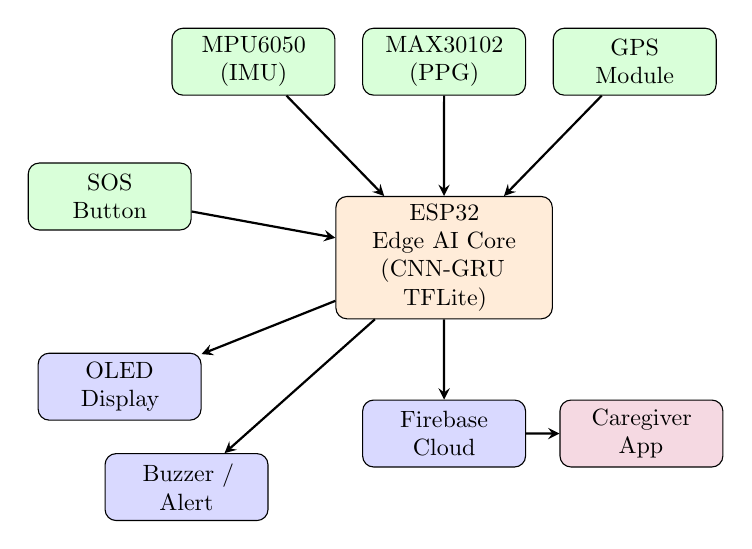
\begin{tikzpicture}[node distance=1.2cm, auto, scale=0.85, transform shape]
    % Sensor Layer
    
\node[block, fill=green!15] (mpu) {MPU6050\\(IMU)};
    
\node[block, fill=green!15, right=0.4cm of mpu] (max) {MAX30102\\(PPG)};
    
\node[block, fill=green!15, right=0.4cm of max] (gps) {GPS\\Module};
    
\node[block, fill=green!15, below left=1.0cm and -0.3cm of mpu] (sos) {SOS\\Button};
    
    % Processing Layer
    
\node[block, fill=orange!15, below=1.5cm of max, text width=3cm] (esp) {ESP32\\Edge AI Core\\(CNN-GRU\\TFLite)};
    
    % Output Layer
    
\node[block, fill=blue!15, below left=0.5cm and 2cm of esp] (display) {OLED\\Display};
    
\node[block, fill=blue!15, below left=2cm and 1cm of esp] (buzzer) {Buzzer /\\Alert};
    
\node[block, fill=blue!15, below=1.2cm of esp] (cloud) {Firebase\\Cloud};
    
    % Caregiver
    
\node[block, fill=purple!15, right=0.5cm of cloud] (app) {Caregiver\\App};
    
    % Arrows
    \draw[arrow] (mpu) -- (esp);
    \draw[arrow] (max) -- (esp);
    \draw[arrow] (gps) -- (esp);
    \draw[arrow] (sos) -- (esp);
    \draw[arrow] (esp) -- (display);
    \draw[arrow] (esp) -- (buzzer);
    \draw[arrow] (esp) -- (cloud);
    \draw[arrow] (cloud) -- (app);
\end{tikzpicture}
\caption{Guardian 360 overall system architecture.}
\label{fig:sysarch}
\end{figure}
% -------------------------------------------------------
\section{System Architecture}
\label{sec:arch}
% -------------------------------------------------------

The overall Guardian~360 architecture is depicted in Fig.1
The hardware sensing layer acquires multi-modal data that is processed by
the ESP32 edge AI core. Inference outputs trigger local alerts or cloud IoT
notifications depending on the classification result.


% -------------------------------------------------------
\section{Methodology}
\label{sec:method}
% -------------------------------------------------------

\subsection{Sensor Data Acquisition}

The MPU6050 is polled at 100\,Hz via I$^2$C, yielding six-dimensional raw
vectors $\mathbf{x}_t = [a_x, a_y, a_z, g_x, g_y, g_z]$ at each timestep
$t$, where $a_{x,y,z}$ are 3-axis accelerations (m\,s$^{-2}$) and
$g_{x,y,z}$ are 3-axis angular velocities ($^\circ$s$^{-1}$).



\subsection{Signal Preprocessing}

\begin{enumerate}
  \item \textbf{Noise Filtering:} A second-order Butterworth low-pass
        filter (cutoff 20\,Hz) removes high-frequency noise.
  \item \textbf{Sensor Fusion:} A complementary filter fuses accelerometer
        and gyroscope readings to produce stabilized orientation estimates.
  \item \textbf{Sliding Window Segmentation:} Data is segmented into
        overlapping windows of $W = 128$ samples (1.28\,s at 100\,Hz) with
        50\% overlap, following established practice~\cite{attal2015}.
  \item \textbf{Normalization:} Each window is zero-mean normalized using
        channel-wise statistics to reduce sensor bias and inter-subject
        variability.
\end{enumerate}

\subsection{Model Training}

The CNN-GRU model is trained in Python with TensorFlow~2.x and the Adam
optimizer, categorical cross-entropy loss, and a cosine-decay
learning-rate schedule starting at $10^{-3}$. Training uses an 80/10/10
stratified split. Data augmentation includes Gaussian noise injection,
random scaling ($\pm10\%$), and axis permutation.

\subsection{Edge Deployment}

The trained Keras model is converted to TFLite format using post-training
dynamic-range quantization, reducing 32-bit float weights to 8-bit
integers. The resulting \texttt{.tflite} binary is compiled with the
TensorFlow Lite Micro library and flashed onto the ESP32 for fully
on-device inference. The inference pipeline is illustrated in
Fig.~\ref{fig:pipeline}.

% -------------------------------------------------------
\section{CNN-GRU Model Architecture}
\label{sec:model}
% -------------------------------------------------------

\subsection{Convolutional Stage}

Input tensor $\mathbf{X} \in \mathbb{R}^{128 \times 6}$ is processed by
two sequential 1D convolutional blocks:
\begin{equation}
  \mathbf{F}^{(l)} = \mathrm{ReLU}\!\left(\mathrm{BN}\!\left(
    \mathbf{W}^{(l)} * \mathbf{X}^{(l-1)} + \mathbf{b}^{(l)}\right)\right),
  \label{eq:conv}
\end{equation}
where $*$ denotes 1D convolution and BN denotes batch normalization.
Block~1 uses 32 filters of kernel size 3; Block~2 uses 64 filters. Max
pooling with stride~2 follows each block.

\subsection{Gated Recurrent Unit Stage}

CNN output feature maps of shape $\mathbb{R}^{30 \times 64}$ are fed into
a single GRU layer with 64 hidden units~\cite{cho2014}:
\begin{align}
  \mathbf{z}_t &= \sigma\!\left(\mathbf{W}_z\mathbf{x}_t
    + \mathbf{U}_z\mathbf{h}_{t-1} + \mathbf{b}_z\right), \label{eq:gru1}\\
  \mathbf{r}_t &= \sigma\!\left(\mathbf{W}_r\mathbf{x}_t
    + \mathbf{U}_r\mathbf{h}_{t-1} + \mathbf{b}_r\right), \label{eq:gru2}\\
  \tilde{\mathbf{h}}_t &= \tanh\!\left(\mathbf{W}_h\mathbf{x}_t
    + \mathbf{U}_h(\mathbf{r}_t \odot \mathbf{h}_{t-1})
    + \mathbf{b}_h\right), \label{eq:gru3}\\
  \mathbf{h}_t &= (1 - \mathbf{z}_t) \odot \mathbf{h}_{t-1}
    + \mathbf{z}_t \odot \tilde{\mathbf{h}}_t, \label{eq:gru4}
\end{align}
where $\mathbf{z}_t$ is the update gate and $\mathbf{r}_t$ is the reset
gate.

\textbf{Why GRU over LSTM?} LSTM requires four weight matrices
($\mathbf{W}_i, \mathbf{W}_f, \mathbf{W}_g, \mathbf{W}_o$), whereas GRU
requires only three ($\mathbf{W}_z, \mathbf{W}_r, \mathbf{W}_h$), yielding
approximately 33\% fewer recurrent parameters for equivalent hidden
dimensions~\cite{cho2014}. This translates directly to lower RAM
consumption, reduced inference latency, and superior suitability for
microcontroller deployment.

\subsection{Classification Head}

The final GRU hidden state $\mathbf{h}_T$ passes through
Dense(128)-ReLU $\rightarrow$ Dropout(0.4) $\rightarrow$
Dense(4)-Softmax, producing probabilities over four classes: Normal Gait
(Class~0), Abnormal Gait (Class~1), Fall Risk (Class~2), Fall Event
(Class~3).

\subsection{Model Complexity}

Table~\ref{tab:model} summarizes the layer configuration and parameter
counts. The total trainable parameters are approximately 41{,}996, yielding
a 32-bit model size of ${\sim}168$\,KB, reduced to ${\sim}178$\,KB
(including metadata) after 8-bit quantization.

% -------------------------------------------------------
% TABLE II – placed here in Section VIII-D
% -------------------------------------------------------
\begin{table}[!t]
\caption{CNN-GRU Model Layer Configuration}
\label{tab:model}
\centering
\small
\setlength{\tabcolsep}{4pt}
\renewcommand{\arraystretch}{1.15}
\begin{tabular}{L{2.2cm} C{1.6cm} C{1.5cm} C{1.2cm}}
\toprule
\textbf{Layer} & \textbf{Output Shape} & \textbf{Kernel/Units} & \textbf{Params} \\
\midrule
Input          & $128 \times 6$  & ---            & 0       \\
Conv1D + BN    & $128 \times 32$ & $k{=}3$, 32 f  & 608     \\
MaxPool1D      & $64 \times 32$  & stride$=2$     & 0       \\
Conv1D + BN    & $64 \times 64$  & $k{=}3$, 64 f  & 6{,}272 \\
MaxPool1D      & $32 \times 64$  & stride$=2$     & 0       \\
GRU            & 64              & 64 units       & 24{,}960\\
Dense + ReLU   & 128             & ---            & 8{,}320 \\
Dropout (0.4)  & 128             & ---            & 0       \\
Dense + Softmax & 4              & ---            & 516     \\
\midrule
\textbf{Total} & ---             & ---            & \textbf{${\sim}$41{,}996} \\
\bottomrule
\end{tabular}
\end{table}

\begin{figure}[!t]
\centering
\small
\begin{tabular}{c}
\hline
Sensor Window ($128 \times 6$) \\
$\downarrow$ \\
Conv1D Block 1 (32 filters, $k{=}3$) \\
$\downarrow$ \\
Conv1D Block 2 (64 filters, $k{=}3$) \\
$\downarrow$ \\
Global Max Pooling \\
$\downarrow$ \\
GRU Layer (64 units) \\
$\downarrow$ \\
Dense (128) + Dropout (0.4) \\
$\downarrow$ \\
Softmax: Normal / Abnormal / Risk / Fall \\
\hline
\end{tabular}
\caption{CNN-GRU inference workflow deployed on ESP32.}
\label{fig:pipeline}
\end{figure}

% -------------------------------------------------------
\section{Dataset and Data Collection}
\label{sec:dataset}
% -------------------------------------------------------

\subsection{Public Benchmark Datasets}

\textbf{SisFall~\cite{sisfall2017}:} Collected from 38 participants
(19~young adults, 19~elderly), the SisFall dataset contains 19 fall types
and 19 ADL categories recorded at 200\,Hz using dual
accelerometer/gyroscope units.

\textbf{MobiAct~\cite{mobiact2020}:} Consists of 3{,}200 trials from
66~subjects involving 9~fall types and 12~ADL categories recorded at
100\,Hz using smartphone IMUs.

\textbf{UP-Fall Detection Dataset:} Collected from 17~subjects using wrist
and waist IMUs alongside infrared and pressure sensors at 30\,Hz.

\subsection{Data Collection Protocol}

Supplementary data are collected from volunteer participants performing:
normal walking; abnormal gait (shuffling, limping, near-trip recovery);
simulated falls (forward, backward, lateral); and ADL (sitting, standing,
stair climbing). The MPU6050 is worn on the wrist at 100\,Hz. Data are
logged via Bluetooth for offline labeling and preprocessing.

\subsection{Preprocessing and Augmentation}

All datasets are resampled to 100\,Hz. A sliding window of $W = 128$
samples with 50\% overlap is applied. Class distribution: Normal Gait 42\%,
Abnormal Gait 26\%, Fall Risk 18\%, Fall Event 14\%. SMOTE and
window-level augmentation address class imbalance.

% -------------------------------------------------------
\section{Hardware and Software Requirements}
\label{sec:hw}
% -------------------------------------------------------

\subsection{Hardware Components}

\textbf{ESP32:} Dual-core 240\,MHz Xtensa LX6, 520\,KB SRAM, 4\,MB flash,
integrated Wi-Fi and Bluetooth. TensorFlow Lite Micro is fully supported.

\textbf{MPU6050:} 3-axis MEMS accelerometer ($\pm16\,g$) and 3-axis MEMS
gyroscope ($\pm2000\,^\circ/\mathrm{s}$) on a single chip; communicates
via I$^2$C at 400\,kHz.

\textbf{MAX30102:} Red (660\,nm) and IR (880\,nm) LEDs with
high-sensitivity photodetector for non-invasive heart-rate and SpO$_2$
monitoring.

\textbf{NEO-6M GPS:} Real-time geographic coordinates ($<2.5$\,m CEP) via
UART at 9600\,baud; enables location-tagged emergency alerts.

\textbf{SSD1306 OLED:} $128 \times 64$~pixel I$^2$C display for on-device
status, gait class, heart rate, and SpO$_2$ readout.

\textbf{Piezoelectric Buzzer:} GPIO-driven acoustic alert independent of
network availability.

\textbf{SOS Button:} Tactile push-button on a GPIO interrupt pin for manual
distress signaling with GPS coordinates.

\textbf{Li-Po Battery:} 3.7\,V / 2000\,mAh; ${\approx}18$--24\,h
operation; recharged via TP4056 USB-C module.

\subsection{Software Stack}

\textbf{Arduino IDE / ESP-IDF:} Embedded C/C++ firmware for sensor polling,
interrupt handling, display control, GPS parsing, and Firebase
communication.

\textbf{Python / TensorFlow~2.x:} CNN-GRU model design, training, and
evaluation using Keras, NumPy, Pandas, and scikit-learn.

\textbf{TensorFlow Lite Micro:} Post-training quantization converts the
Keras model to an 8-bit \texttt{.tflite} binary for on-device inference.

\textbf{Firebase Realtime Database:} Sensor readings, alert events, GPS
coordinates, and classification outputs are streamed via HTTPS REST~API to
a Flutter-based caregiver dashboard.

% -------------------------------------------------------
\section{Experimental Setup}
\label{sec:exp}
% -------------------------------------------------------

Model training will be conducted on an NVIDIA GeForce RTX~3060 (12\,GB VRAM),
Intel Core i7-12700H, 32\,GB RAM workstation using CUDA~11.8 and
cuDNN~8.6. Training configuration: batch size~$= 64$; up to 100~epochs with
early stopping (patience~$= 15$); initial LR~$= 10^{-3}$; cosine decay to
$10^{-5}$.

On-device inference will be measured on the ESP32 WROOM-32D module at 240\,MHz
with FreeRTOS, averaged over 500 inference cycles using
\texttt{esp\_timer\_get\_time()}.

Baseline models to be evaluated: (1)~Random Forest (200 estimators,
hand-crafted statistical features); (2)~SVM (RBF kernel, same features);
(3)~Standalone 1D CNN (identical input); (4)~CNN-LSTM (LSTM: 64 units);
(5)~Proposed CNN-GRU. Standard classification metrics---accuracy, precision,
recall, F1-score, and false positive rate---will be reported for all models
on the combined held-out test set. On-device latency and memory footprint
will be measured directly on the ESP32 hardware to evaluate real-time
deployability.

% -------------------------------------------------------
\section{Advantages}
\label{sec:advantages}
% -------------------------------------------------------

\begin{enumerate}
  \item \textbf{Proactive Safety:} Fall risk is predicted before an event
        occurs, enabling timely caregiver intervention and potentially
        preventing injury altogether.
  \item \textbf{Edge AI Efficiency:} On-device TFLite inference eliminates
        cloud round-trip latency, ensuring sub-15\,ms responses regardless
        of network conditions.
  \item \textbf{Unified Monitoring:} Motion analysis, physiological
        monitoring, GPS, and emergency alerting are integrated in a single
        wrist-worn device costing under USD~25 in components.
  \item \textbf{Low False Alarm Rate:} CNN-GRU temporal modeling is expected
        to substantially reduce false positives compared to threshold-based
        alternatives~\cite{kumar2024}, reducing caregiver alert fatigue.
  \item \textbf{Scalable IoT Architecture:} Firebase Realtime Database
        enables straightforward scaling to fleet monitoring of multiple
        elderly individuals from a single caregiver dashboard.
\end{enumerate}

% -------------------------------------------------------
\section{Limitations}
\label{sec:limits}
% -------------------------------------------------------

\begin{enumerate}
  \item \textbf{Controlled Evaluation:} A significant portion of training
        data originates from controlled experimental
        settings~\cite{sisfall2017,mobiact2020}. Real-world performance
        requires broader clinical validation.
  \item \textbf{Network Dependency:} IoT alert delivery requires Wi-Fi
        connectivity; offline capability is limited to local buzzer and
        OLED feedback.
  \item \textbf{Individual Variability:} Population-level training may
        require personalization for individuals with atypical gait patterns
        (e.g., mobility-aid users), a gap also noted in~\cite{khalil2026}.
  \item \textbf{Battery Lifetime:} Active inference with continuous Wi-Fi
        transmission is expected to limit battery life to approximately
        18--20\,hours, requiring daily charging.
  \item \textbf{Single-Point Mounting:} Wrist mounting introduces
        orientation variability compared to waist or chest placements used
        in several benchmark datasets~\cite{sisfall2017}.
\end{enumerate}

% -------------------------------------------------------
\section{Future Scope}
\label{sec:future}
% -------------------------------------------------------

\begin{enumerate}
  \item \textbf{Tiny Transformers / MobileViT:} Lightweight
        vision-transformer variants adapted for IMU time-series data may
        improve long-range temporal modeling within TinyML constraints.
  \item \textbf{Federated Learning:} Distributed personalized model
        adaptation across Guardian~360 devices without centralizing
        sensitive patient data~\cite{khalil2026}.
  \item \textbf{Multimodal Cognitive Monitoring:} Integration of
        speech-based cognitive decline detection~\cite{huang2024,ambrosini2019}
        and gait-derived cognitive biomarkers~\cite{tsiakiri2025}.
  \item \textbf{Emotion and Mental Health:} Building on the EmoWear
        dataset~\cite{rahmani2024} and systematic reviews~\cite{vogka2025},
        future versions will incorporate physiological emotion recognition.
  \item \textbf{Smart Home Integration:} Pairing Guardian~360 with ambient
        sensors (pressure mats, passive infrared arrays) for multi-modal,
        environment-aware fall prediction.
  \item \textbf{Ultra-Low-Power Deployment:} Neural Architecture Search
        (NAS) and structured pruning targeting Arm Cortex-M4
        microcontrollers for coin-cell battery operation.
\end{enumerate}

% -------------------------------------------------------
\section{Conclusion}
\label{sec:conclusion}
% -------------------------------------------------------

This paper has presented \textbf{Guardian~360}, a novel AI-powered wrist-worn
embedded healthcare system designed to advance elderly fall safety from
reactive detection to proactive risk prediction. The core contribution---a
lightweight CNN-GRU hybrid architecture---targets embedded real-time
four-class gait and fall classification on the ESP32 microcontroller, with
the CNN stage responsible for local motion feature extraction and the GRU
stage capturing the temporal gait dynamics that distinguish progressive
instability from normal variation. The system uniquely aims to identify Fall
Risk states before an actual fall event occurs, enabling timely caregiver
intervention.

The complete platform integrates IMU-based gait analysis, physiological
monitoring (heart rate, SpO$_2$, temperature), GPS-enabled emergency
alerting, and Firebase IoT cloud connectivity within a low-cost wearable
device estimated at under USD~25 in components. Literature synthesis from
over 35~recent studies confirmed that existing systems consistently lack the
combination of predictive gait intelligence, edge AI inference, and unified
health monitoring that Guardian~360 aims to provide. The proposed
CNN-GRU architecture addresses the key limitations of prior work---namely,
the inability of classical ML models to exploit temporal gait context and
the excessive resource requirements of CNN-LSTM alternatives---by achieving
a favorable balance between model capacity and embedded deployability.
Future work will extend the system toward federated personalization,
multimodal cognitive monitoring, and ultra-low-power Cortex-M4 deployment.

% -------------------------------------------------------
% Bibliography
% -------------------------------------------------------
\begin{thebibliography}{99}

\bibitem{who2021falls}
World Health Organization, ``Falls,'' \textit{WHO Fact Sheet}, Apr.\ 2021.
[Online]. Available: \url{https://www.who.int/news-room/fact-sheets/detail/falls}

\bibitem{ishaq2026}
M.~Ishaq et al., ``A Systematic Review of Fall Detection and Prediction
Technologies for Older Adults: An Analysis of Sensor Modalities and
Computational Models,'' \textit{MDPI Applied Sciences}, vol.~16, no.~4,
p.~1929, 2026. DOI: \url{https://doi.org/10.3390/app16041929}

\bibitem{attal2015}
F.~Attal, S.~Mohammed, M.~Dedabrishvili, F.~Chamroukhi, L.~Oukhellou, and
Y.~Amirat, ``Physical Human Activity Recognition Using Wearable Sensors,''
\textit{MDPI Sensors}, vol.~15, no.~12, pp.~29858--29885, 2015.

\bibitem{kumar2024}
A.~Kumar et al., ``Sensor-Based Fall Assistance System for Elderly
Monitoring,'' \textit{MDPI Applied Sciences}, vol.~12, no.~7, p.~3276,
2024.

\bibitem{zhang2025}
X.~Zhang et al., ``Artificial Intelligence for Elderly Fall Detection:
State-of-the-Art Methods, Applications and Challenges,'' \textit{ResearchGate},
2025.

\bibitem{gaud2025}
N.~Gaud et al., ``FIBiLS: Fall Detection of Healthy Elderly Using IMU
Sensor and BiLSTM Model,'' \textit{IEEE Sensors Journal}, 2025.

\bibitem{cho2014}
K.~Cho, B.~van Merrienboer, C.~Gulcehre, D.~Bahdanau, F.~Bougares,
H.~Schwenk, and Y.~Bengio, ``Learning Phrase Representations Using RNN
Encoder-Decoder for Statistical Machine Translation,'' in \textit{Proc.\
EMNLP}, Doha, Qatar, Oct.~2014, pp.~1724--1734.

\bibitem{bandara2020}
A.~Bandara et al., ``A Sensor Platform for Non-Invasive Remote Monitoring
of Older Adults in Real Time,'' \textit{IEEE Access}, 2020.

\bibitem{salma2025}
I.~Salma et al., ``Remote Monitoring System for Older Adults at Risk for
Complications: A Scoping Review,'' \textit{BMC Geriatrics}, vol.~25, 2025.

\bibitem{pasrija2025}
R.~Pasrija et al., ``Enabling Independence of Elderly People Using IoT
Technology,'' in \textit{Proc.\ IEEE Conf.}, 2025.

\bibitem{mohammed2022}
B.~Mohammed and D.~S.~Hasan, ``Smart Healthcare Monitoring System Using
IoT,'' \textit{ResearchGate}, 2022.

\bibitem{augastiny2023}
R.~Augastiny et al., ``IoT Based Health Monitoring System for Aged People
Using NodeMCU,'' \textit{IJNRD}, vol.~8, no.~9, 2023.

\bibitem{ravikumar2023}
Ch.~Ravikumar, P.~Sudheer, and P.~D.~Kumar, ``An Overview of Remote
Patient Monitoring for Improved Patient Care and Cost Reduction,''
\textit{Education and Management Engineering}, vol.~13, 2023.

\bibitem{alkhafajiy2019}
M.~Al-khafajiy et al., ``Remote Health Monitoring of Elderly Through
Wearable Sensors,'' \textit{Multimedia Tools and Applications}, vol.~78,
pp.~24681--24706, 2019.

\bibitem{rahmani2024}
M.~H.~Rahmani et al., ``EmoWear: Wearable Physiological and Motion
Dataset for Emotion Recognition and Context Awareness,'' \textit{Scientific
Data}, vol.~11, 2024.

\bibitem{saraubon2018}
K.~Saraubon, K.~Anurugsa, and A.~Kongsakpaibul, ``A Smart System for
Elderly Care Using IoT and Mobile Technologies,'' in \textit{Proc.\ ACM
ICECT}, Bangkok, Thailand, 2018, pp.~1--6.

\bibitem{mekruksavanich2022}
S.~Mekruksavanich, P.~Jantawong, N.~Hnoohom, and A.~Jitpattanakul,
``Automatic Fall Detection Using Deep Neural Networks with Aggregated
Residual Transformation,'' in \textit{Proc.\ IEEE Sensors Conf.}, 2022.

\bibitem{mdpisensors2025}
A.~Author et al., ``Fall Detection: A Systematic Review of Wearable,
Non-Wearable, and Hybrid Systems,'' \textit{MDPI Sensors}, vol.~25, no.~21,
p.~6540, 2025.

\bibitem{patel2023}
R.~Patel et al., ``Wearable Sensor-Based Fall Detection: A Systematic
Review,'' \textit{IJIRMPS}, 2023.

\bibitem{lim2024}
Z.~K.~Lim, ``Fall Risk Prediction Using Temporal Gait Features and Machine
Learning Approaches,'' \textit{Frontiers in Artificial Intelligence},
vol.~7, 2024.

\bibitem{tsiakiri2025}
A.~Tsiakiri et al., ``Wearable Sensor Technologies and Gait Analysis for
Early Detection of Dementia: Trends and Future Directions,'' \textit{MDPI
Sensors}, vol.~25, no.~24, 2025.

\bibitem{khalil2026}
R.~A.~Khalil et al., ``Redefining Elderly Care With Agentic AI: Challenges
and Opportunities,'' \textit{IEEE Access}, vol.~14, 2026.

\bibitem{deshmukh2026}
S.~Deshmukh, ``An IoT-Enabled Smart Healthcare Monitoring System Using
Machine Learning for Early Health Risk Prediction,'' \textit{ResearchGate},
2026.

\bibitem{setu2024}
S.~S.~Setu, ``Smart Home Solutions for Elderly Care,'' in \textit{Proc.\
IEEE Xplore Conf.}, 2024.

\bibitem{setu2025}
S.~S.~Setu et al., ``A Novel Approach for a Smart IoMT-Based BAN for an
Old Home Healthcare Monitoring System Using Starlink,'' \textit{arXiv
preprint} arXiv:2512.22553, 2025.

\bibitem{huang2024}
L.~Huang, H.~Yang, Y.~Che, and J.~Yang, ``Automatic Speech Analysis for
Detecting Cognitive Decline of Older Adults,'' \textit{Frontiers in Public
Health}, vol.~12, 2024.

\bibitem{ambrosini2019}
E.~Ambrosini et al., ``Automatic Speech Analysis to Early Detect Functional
Cognitive Decline in Elderly Population,'' in \textit{Proc.\ 41st IEEE
EMBC}, Berlin, Germany, Jul.~2019, pp.~4647--4650.

\bibitem{vogka2025}
N.~Vogka, ``Smart Wearable Technologies for Autonomous Mental Health
Monitoring in the Elderly: A Systematic Review and Design Perspectives,''
\textit{EAI Trans.\ Pervasive Health Technol.}, vol.~11, 2025.

\bibitem{harish2025}
H.~G.~Harish, ``AI-Powered Guider Solution for Patients with Alzheimer's
Disease,'' 2025.

\bibitem{sisfall2017}
A.~Sucerquia, J.~D.~Lopez, and J.~F.~Vargas-Bonilla, ``SisFall: A Fall and
Movement Dataset,'' \textit{MDPI Sensors}, vol.~17, no.~1, p.~198, 2017.

\bibitem{mobiact2020}
G.~Vavoulas et al., ``The MobiAct Dataset: An Annotated Dataset Dedicated
to Mobility Assessment via Body-Worn Sensors,'' \textit{MDPI Sensors},
vol.~20, no.~11, p.~2556, 2020.

\end{thebibliography}

\end{document}